\chapter{Програм хангамж}

Энэ бүлэгт өөрийн ажлын судалгаан дээр үндэслэн өгөгдөл боловсруулах, сан үүсгэхээр хөгжүүлсэн програмууд болон тэдгээрийг хэрхэн ашиглах талаар авч үзнэ. Энэхүү ажил нь програмтай судалгаа буюу судалгаа голлосон, шаардлагтай байдлаар туслах програмуудыг хөгжүүлсэн учир удирдагч багшийн зөвлөснөөр шинжилгээ, зохиомж шаардлагагүйгээр CLI буюу комманд мөр интерфэйстэйгээр хийж гүйцэтгэсэн.

\section{Sanitizer}
\label{section:sanitizer}

Энэхүү жижиг програм нь маягтаас боловсруулалт хийн салган авсан тэмдэгтүүд давхардсан эсэхийг зурган файлын hash -г тооцоолон (Код \ref{lst:collect_hash}) цэвэрлэдэг бөгөөд маш олон тооны зургууд дээр боловсруулалт хийж байгаа учир тооцооллын хугацааг бага байлгахын тулд Python 3 \cite{python} дээр нэмэгдсэн асинхрон тооцооллын \texttt{concurrent.futures} санг ашигласан.

\begin{figure}[ht]
	\begin{subfigure}{0.5\textwidth}
		\centering
		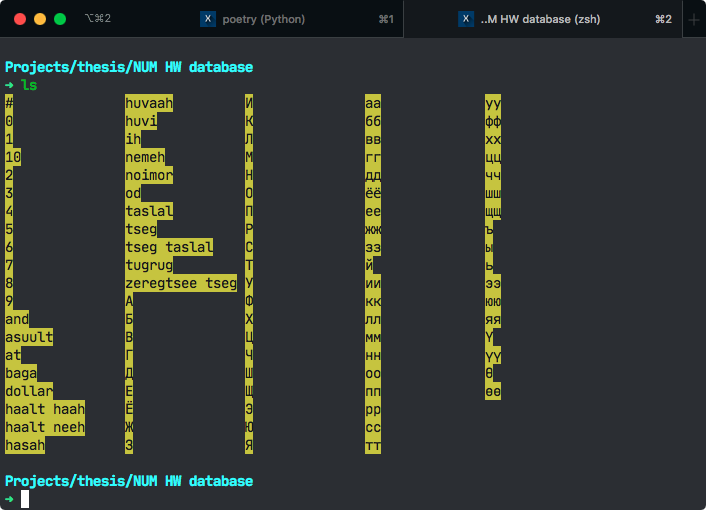
\includegraphics[width=0.9\linewidth]{images/sanitizer_input}
		\caption{Оролт}
		\label{fig:sanitizer_input}
	\end{subfigure}
	\begin{subfigure}{0.5\textwidth}
		\centering
		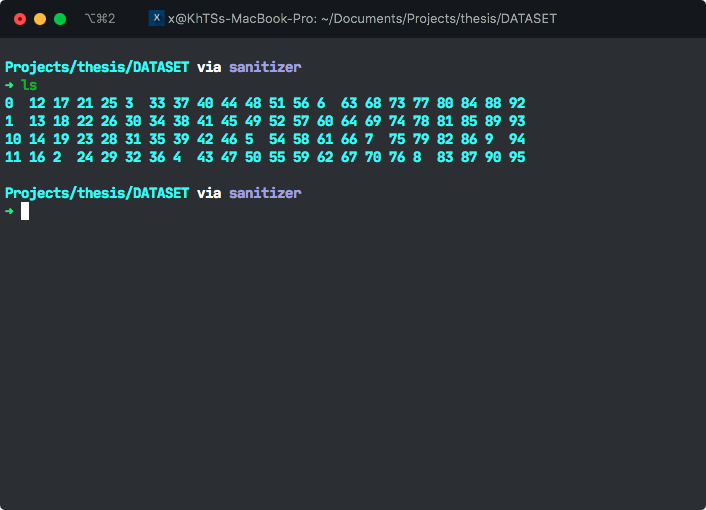
\includegraphics[width=0.9\linewidth]{images/sanitizer_output}
		\caption{Гаралт}
		\label{fig:sanitizer_output}
	\end{subfigure}
	\caption{Sanitizer -г ашиглан нийт 97 тэмдэгт бүхий нийт 255576 зургаас давхардсанг ялгах үеийн оролт болон гаралт}
	\label{fig:sanitizer}
\end{figure}

\begin{lstlisting}[caption={Параметраар өгөгдсөн файлын нэрээр зургийг уншин тэмдэгтийн түлхүүр (label), зургийн нэр, hash утгыг агуулсан tuple буцаах функц}, label={lst:collect_hash}, language=Python]
def fingerprint(cls, filename):
		try:
				return (
						cls.LABELS[
								str(filename.parent.stem).split("/")[-1]
						]["id"],
						filename,
						hashlib.md5(open(filename, "rb").read()).hexdigest(),
				)
		except KeyError:
				print(f"Ignored: {str(filename.parent.stem).split('/')[-1]}")

\end{lstlisting}

Удирдагч багшийн “Гинжин кодын аргаар Монгол хэлний гар бичмэл танилт” \cite{mongolian-htr-using-chain-code} судалгааны ажлын хүрээнд цуглуулсан хүмүүсийн гар бичмэлээс ялган ангилсан 97 ялгаатай тэмдэгтүүдээс бүрдэх нийт 255576 ширхэг зураг бүхий өгөгдлийг (Зураг \ref{fig:sanitizer_input}) боловсруулан ашиглахдаа эхлээд давхардсан зургуудыг арилгах шаардлагатай болсон ба үр дүнд давхардалгүй 103592 зургийг харгалзах тэмдэгтийн хавтас бүрт хадгалсан (Зураг \ref{fig:sanitizer_output}) байдлыг Зураг \ref{fig:sanitizer_result} -ээс харж болно. Үр дүнд үүссэн хавтаснууд (Зураг \ref{fig:sanitizer_output}) болон тэдгээрийн нэр нь \texttt{config.json}\footnote{\url{https://github.com/khasbilegt/sanitizer/blob/master/config.json}} болон \texttt{labels.json}\footnote{\url{https://github.com/khasbilegt/sanitizer/blob/master/labels.json}} -оос хамаарах ба өгөгдөл нь тусгай тэмдэгтүүдийг ч мөн агуулж буй учир тэмдэгтийн түлхүүрээр хавтсыг нэрлэх боломжгүй. Тийм учраас тэмдэгтийн түлхүүрийг 0 -ээс эхэлсэн бүхэл тоогоор дугаарласан бөгөөд ямар дугаар ямар тэмдэгттэй харгалзаж буй мэдээллийг дээрх JSON файлуудад хадгалсан.

\begin{figure}[ht]
	\centering
	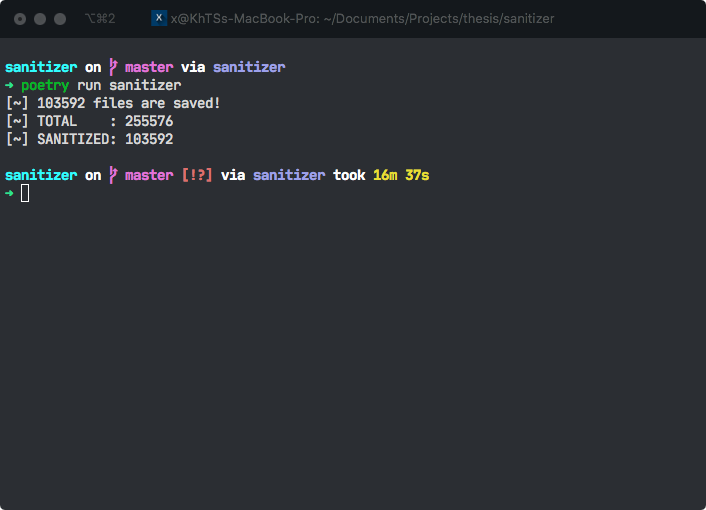
\includegraphics[width=0.9\linewidth]{images/sanitizer}
	\caption{Sanitizer програмын жишээ үр дүн}
	\label{fig:sanitizer_result}
\end{figure}

\section{NUMiner}

NUMiner нь гараар бөглөгдсөн маягтын зургийг боловсруулахаас тэмдэгтүүдийг ялган авч зураг болгоод MNIST -тэй адил IDX файл форматтай болгон хувиргах хүртэлх бүх боловсруулалтуудыг гүйцэтгэж байгаа бөгөөд \textit{Шаардлага №\ref{criteria:5}} -д тодорхойлсоны дагуу програмыг PyPi\footnote{NUMiner --- \url{https://pypi.org/project/numiner}} дээр байрлуулсан. Ингэснээр ямар ч хүн \texttt{pip}\footnote{Pip --- \url{https://github.com/pypa/pip}}, \texttt{pipenv}\footnote{Pipenv --- \url{https://github.com/pypa/pipenv}}, \texttt{poetry}\footnote{Poetry --- \url{https://python-poetry.org/}} гэх мэт Python хэлний ямар ч багц удирдлагын програмыг ашиглан амархан авч ашиглах боломжтой.

Энэхүү програм нь CLI буюу комманд мөр интерфэйстэй учир системийн терминал эсвэл түүнтэй холбоотой програмыг ашиглан ажиллуулна. Нийтлэг ашиглах тохиолдол нь тодорхой нэг маягтыг оролтонд өгч боловсруулах эсвэл олон тооны маягтуудыг агуулж буй хавтасны замыг оролтонд өгч боловсруулалт хийх байх бөгөөд \texttt{-s, --sheet} коммандуудыг дараах байдлаар ашиглана.

\begin{lstlisting}[caption={NUMiner --- нэг маягтыг боловсруулах комманд}, label={lst:numiner_sheet}, language=bash, numbers=none]
$ numiner -s data/INPUT/SHEET_10_10_00001.jpg data/OUTPUT
\end{lstlisting}

\begin{lstlisting}[caption={NUMiner --- олон маягтуудыг нэг дор боловсруулах комманд буюу маягтуудыг агуулж буй хавтсын замыг зааж өгөх}, label={lst:numiner_sheets}, language=bash, numbers=none]
$ numiner -s data/INPUT data/OUTPUT
\end{lstlisting}

Код \ref{lst:numiner_sheets} -н үр дүнд \texttt{data/INPUT} хавтас дотроос \texttt{PNG, JPG, JPEG} зургуудыг олж, файлын нэр нь \texttt{SHEET} гэж эхэлсэн, хүснэгтийн мөр болон баганы тоог, мөн дугаар оруулсан байгаа эсэхийг шалган
\begin{center}
	\texttt{SHEET\_<row\_count>\_<col\_count>\_<sheet\_id>.<extension>}
\end{center}
цааш боловсруулалтыг гүйцэтгэнэ. Боловсруулалтын үр дүн нь \texttt{data/OUTPUT} хавтас дотор тэмдэгт бүр өөрийн харгалзах дугаартай хавтас дотор
\begin{center}
	\texttt{<sheet\_id>\_<label\_id>\_<datetime>.<extension>}
\end{center}
нэртэйгээр үүснэ.

Код \ref{lst:numiner_sheet} -н ажиллагаа Код \ref{lst:numiner_sheets} -тэй адилхан бөгөөд ганц ялгаа нь оролтын зам нь хавтасных бус яг нэг маягтын зургийг заасан зам учир гаралтанд зөвхөн тухайн маягтын тэмдэгтүүд л боловсруулагдсан байна.

Энэхүү бүлгийн эхний хэсэг \ref{section:sanitizer} -т ашигласантай адилаар магт нь тусгай тэмдэгтүүд агуулж байгаа учир хавтсыг тэмдэгтийн түлхүүрээр хадгалах боломжгүй юм. Маягтын хүснэгтийн нүд бүрийг тодорхой дугаартай харгалзуулан гаралтын үр дүнд харгалзах дугаараар хавтсуудыг үүсгэх ба энэ програм энэ мэдээллийг \texttt{--labels} коммандыг ашиглан тэмдэгтийн түлхүүр болон харгалзах дугаарыг агуулах тохиргооны JSON файлаас дараах байдлаар унших боломжтой. Код \ref{lst:numiner_labels}. JSON файл доторх тохиргооны зохион байгуулалтыг Код \ref{lst:numiner_label_sample} -аас харж болох бөгөөд NUMiner -н файлыг уншиж тохиргоог хийж байгаа кодыг Хавсралт \ref{appendix:handle_config} -с харж болно.

\begin{lstlisting}[caption={NUMiner --- config хавтас доторх labels.json нэртэй файлаас тэмдэгтийн түлхүүрүүдийг ямар дугаартай харгалзуулан хадгалахыг уншиж, data/INPUT доторх маягтуудыг боловсруулан үр дүнг data/OUTPUT дотор хадгал}, label={lst:numiner_labels}, language=bash, numbers=none]
$ numiner --labels config/labels.json -s data/INPUT data/OUTPUT
\end{lstlisting}

\begin{lstlisting}[caption={NUMiner --- labels.json}, label={lst:numiner_label_sample}]
{
	"labels": {
		...,
		"91": "!",
		"92": "?",
		"93": "+",
		"94": "-",
		"95": "/",
		...
	}
}
\end{lstlisting}

Боловсруулалт хийн тэмдэгтийн төрөл бүрт зургаар нь хадгалсны дараа \textit{Шаардлага №\ref{criteria:4}} -н дагуу авч ашиглахад хялбар байх зорилгоор MNIST \cite{mnist} өгөгдлийн хэлбэртэй адил IDX форматтай болгон хувиргана. Ингэхдээ програмын \texttt{convert} коммандыг ашиглах бөгөөд коммандын араас оролтын болон гаралтын замууд, нэг классаас авах өгөгдлийн тоо болон сургалт, тестийн өгөгдлийн харьцаа гэх дөрвөн параметрүүдийг олгон ажиллуулах буюу дараах хэлбэртэй байна. Код \ref{lst:numiner_convert}.

\begin{lstlisting}[caption={NUMiner convert --- <src> доторх тэмдэгтийн төрөл бүрээс <size> ширхэг зургийг авах ба нийт өгөгдлөөс <ratio> хувийг нь (хэрэв ratio бүхэл тоо бол нийт өгөгдлөөс салган авах тестийн өгөгдлийн хувь, train бол бүхэлдээ сургалтын, test бол бүхэлдээ тестийн өгөгдөл гэж тус тус үзнэ)  тестийн өгөгдөлд зориулан боловсруулж <dst> -д хадгална.}, label={lst:numiner_convert}, language=bash, numbers=none]
$ numiner convert <src> <dst> <size> <ratio>
\end{lstlisting}

Код \ref{lst:numiner_convert} жишээнд буй <size> нь 0 байж болох ба энэ тохиолдолд тэмдэгтийн төрөл бүрээс бүх зургийг нь өгөгдөлд оролцуулна. Харин <ratio> буюу тестийн өгөгдлийн харьцаа нь бүхэл тооноос гадна \texttt{train}, \texttt{test} гэх үгнүүд байж болох ба ингэвэл тэмдэгтийн төрөлд зааж өгсөн өгөгдлийг бүхэлд нь сургалтын эсвэл тестийн болгон боловсруулна.